\documentclass[12pt]{article}
\usepackage[a4paper,margin=1in]{geometry}
\usepackage{graphicx}
\usepackage{amsmath}
\usepackage{hyperref}
\usepackage[outputdir=../]{minted}
\usepackage{array}
% for the above code thank the increadble StackExchange forum https://tex.stackexchange.com/questions/531738/minted-environment-not-working-in-overleaf

\begin{document}

%-------------------- Title Page --------------------
\title{Laboratory 1: Circuit Designs and Testing}
\author{Shein Htike \and Brandon Vasquez}
\date{CSC 343 Spring 2025}
\maketitle

\tableofcontents
\clearpage

\section{Exercise A: 8x1 Multiplexer Using Logic Gates}
\subsection{Objective}
The goal of this exercise is to create an 8x1 multiplexer in two ways: using logic gates and using VHDL code.
\subsection{Functionality and Specifications}
\subsubsection{Logic}
The output of the 8×1 multiplexer is given by the following logic equation:

\begin{equation}
\begin{split}
\text{output} =\,& \overline{S_2}\,\overline{S_1}\,\overline{S_0}\,I_0 \ \vee\ \overline{S_2}\,\overline{S_1}\,S_0\,I_1 \ \vee \\[1mm]
                & \overline{S_2}\,S_1\,\overline{S_0}\,I_2 \ \vee\ \overline{S_2}\,S_1\,S_0\,I_3 \ \vee \\[1mm]
                & S_2\,\overline{S_1}\,\overline{S_0}\,I_4 \ \vee\ S_2\,\overline{S_1}\,S_0\,I_5 \ \vee \\[1mm]
                & S_2\,S_1\,\overline{S_0}\,I_6 \ \vee\ S_2\,S_1\,S_0\,I_7 
\end{split}
\end{equation}

In this multiplexer design, we select one of the eight inputs, $I_{0}$ through $I_{7}$ and connect it to a single output based on the binary value of the three select signals, $S_{2}$, $S_{1}$, and $S_{0}$ (with $S_{2}$ being the most significant bit).
\clearpage
\subsubsection{Circut Design}
In order to implement the 8x1 multiplexer, we created this circuit design in Intel Quartus Prime.
This circuit was then compiled into VHDL and imported into ModelSim in order to simulate and test our design. \\

\subsection{Functionality and Specifications}
\begin{figure}[h]
\caption{8x1 multiplexer}
\centering
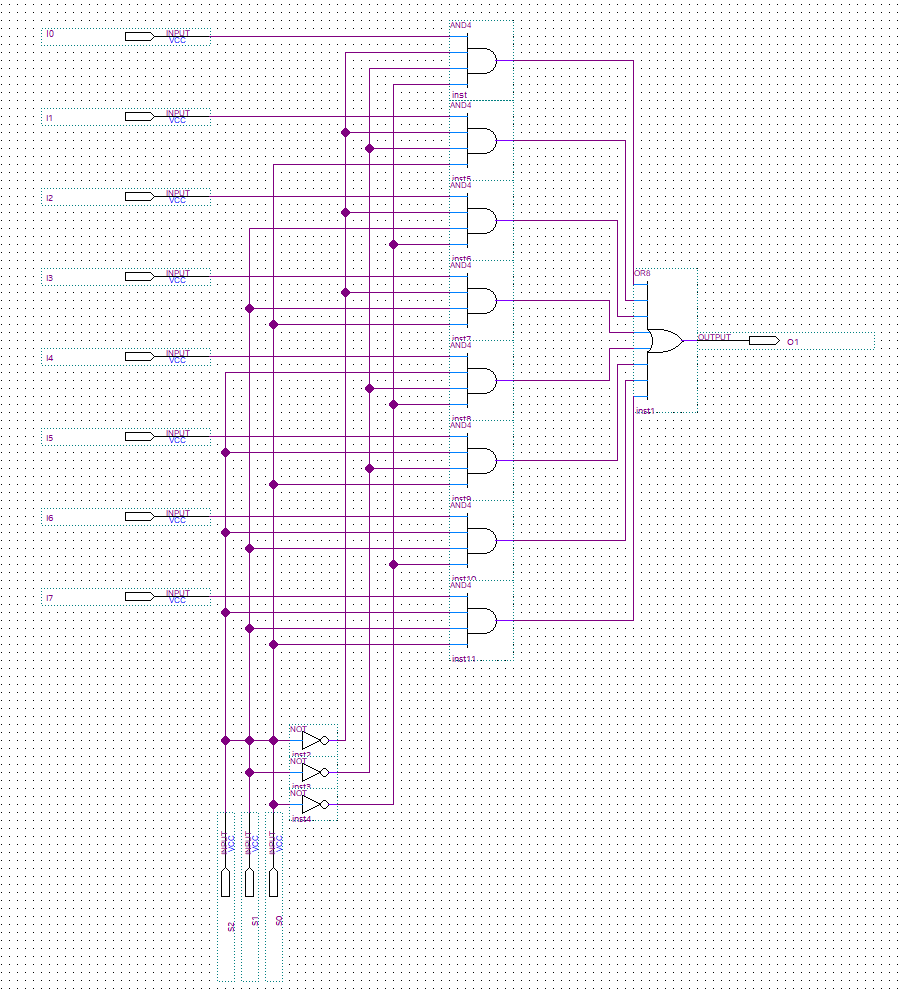
\includegraphics[width=\textwidth]{./diagrams/8x1multiplexer.png}
\end{figure}

\clearpage
\subsubsection{VHDL Code}

\begin{minted}[linenos]{vhdl}
    library IEEE;
    use IEEE.std_logic_1164.all;
    
    entity multiplexer8x1v2 is
        port (
            I : in  std_logic_vector(7 downto 0);
            S : in  std_logic_vector(2 downto 0);
            O : out std_logic
        );
    end multiplexer8x1v2;
    
    architecture Behavioral of multiplexer8x1v2 is
    begin
        with S select
            O <= I(0) when "000",
                 I(1) when "001",
                 I(2) when "010",
                 I(3) when "011",
                 I(4) when "100",
                 I(5) when "101",
                 I(6) when "110",
                 I(7) when "111",
                 '0'    when others;  -- Default case if needed
    end Behavioral;
\end{minted}
\clearpage

\subsection{Simulation}
\clearpage


\section{Exercise B: 1x8 De-Multiplexer Using 1x4 and 1x2 De-Multiplexers}
\subsection{Objective}
The objective of this exercise is to design and write, with structural modelling, a 1x8 de multiplexer using a 1x2 and 1x4 de multiplexer architecture. This would allow for a deeper understanding of designing circuits in Quartis, along with a deeper understanding of the way circuits are derived from both truth tables and boolean functions.

\subsection{Functionality and Specifications}

\begin{figure}[h]
\caption{1x8 demultiplexer from design}
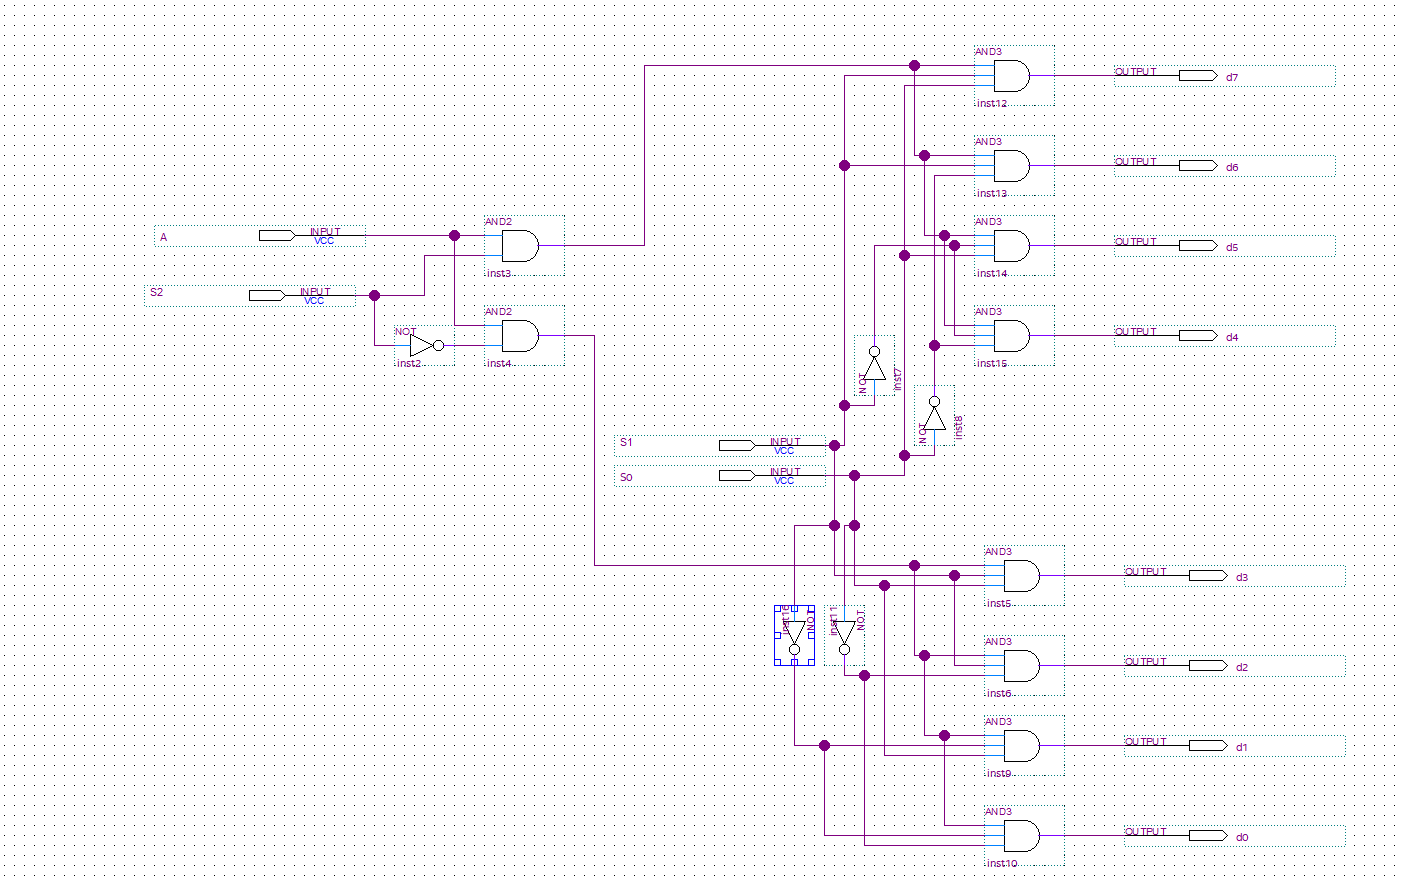
\includegraphics[width=\textwidth]{./diagrams/1x8_demux.png}
\end{figure}
\begin{figure}[h]
    \begin{multline}
        \\i_0 = s_2's_1's_0' \\
        i_1 = s_2's_1's_0 \\
        i_2 = s_2's_1s_0' \\
        i_3 = s_2's_1s_0 \\
        i_4 = s_2s_1's_0' \\
        i_5 = s_2s_1's_0 \\
        i_6 = s_2s_1s_0' \\
        i_7 = s_2s_1s_0 \\
    \end{multline}
    \caption{1x8 demux boolean eq.}
\end{figure}

\noindent The circuit in figure 2 showcases a 1x8 demux which employs 1x2 demux and 1x4 architecture whereby the 1x2 demux is essentially used to select which 1x4 demux will be used and effectively partitioning the selection into two groups of 4.
The idea for structuring the 1x8 was made this way through the boolean function derived from the respective truth table below which the boolean function was then derived from and which shows the way in which the selections for the demux occur. 
\\
\\
\\
\\
\\
\\

\subsubsection{VHDL Code generated from the design file}
\begin{minted}[linenos]{vhdl}
    LIBRARY ieee;
    USE ieee.std_logic_1164.all; 
    
    LIBRARY work;
    
    ENTITY \1x8_demux\ IS 
    	PORT
    	(
    		A :  IN  STD_LOGIC;
    		S2 :  IN  STD_LOGIC;
    		S1 :  IN  STD_LOGIC;
    		S0 :  IN  STD_LOGIC;
    		d0 :  OUT  STD_LOGIC;
    		d1 :  OUT  STD_LOGIC;
    		d2 :  OUT  STD_LOGIC;
    		d7 :  OUT  STD_LOGIC;
    		d6 :  OUT  STD_LOGIC;
    		d5 :  OUT  STD_LOGIC;
    		d4 :  OUT  STD_LOGIC;
    		d3 :  OUT  STD_LOGIC
    	);
    END \1x8_demux\;
    
    ARCHITECTURE bdf_type OF \1x8_demux\ IS 
    
    SIGNAL	SYNTHESIZED_WIRE_17 :  STD_LOGIC;
    SIGNAL	SYNTHESIZED_WIRE_18 :  STD_LOGIC;
    SIGNAL	SYNTHESIZED_WIRE_19 :  STD_LOGIC;
    SIGNAL	SYNTHESIZED_WIRE_20 :  STD_LOGIC;
    SIGNAL	SYNTHESIZED_WIRE_21 :  STD_LOGIC;
    SIGNAL	SYNTHESIZED_WIRE_22 :  STD_LOGIC;
    SIGNAL	SYNTHESIZED_WIRE_11 :  STD_LOGIC;
    
    
    BEGIN 
    
    
    
    d0 <= SYNTHESIZED_WIRE_17 AND SYNTHESIZED_WIRE_18 AND SYNTHESIZED_WIRE_19;
    
    
    SYNTHESIZED_WIRE_19 <= NOT(S0);
    
    
    
    d7 <= SYNTHESIZED_WIRE_20 AND S1 AND S0;
    
    
    d6 <= SYNTHESIZED_WIRE_20 AND S1 AND SYNTHESIZED_WIRE_21;
    
    
    d5 <= SYNTHESIZED_WIRE_20 AND SYNTHESIZED_WIRE_22 AND S0;
    
    
    d4 <= SYNTHESIZED_WIRE_20 AND SYNTHESIZED_WIRE_22 AND SYNTHESIZED_WIRE_21;
    
    
    SYNTHESIZED_WIRE_18 <= NOT(S1);
    
    
    
    SYNTHESIZED_WIRE_11 <= NOT(S2);
    
    
    
    SYNTHESIZED_WIRE_20 <= A AND S2;
    
    
    SYNTHESIZED_WIRE_17 <= A AND SYNTHESIZED_WIRE_11;
    
    
    d3 <= SYNTHESIZED_WIRE_17 AND S1 AND S0;
    
    
    d2 <= SYNTHESIZED_WIRE_17 AND S1 AND SYNTHESIZED_WIRE_19;
    
    
    SYNTHESIZED_WIRE_22 <= NOT(S1);
    
    
    
    SYNTHESIZED_WIRE_21 <= NOT(S0);
    
    
    
    d1 <= SYNTHESIZED_WIRE_17 AND SYNTHESIZED_WIRE_18 AND S0;
    
    
    END bdf_type;

\end{minted}
\subsubsection{VHDL Code testbench from generated design file}
\begin{minted}[linenos]{vhdl}
    library IEEE;
use IEEE.STD_LOGIC_1164.ALL;
use IEEE.STD_LOGIC_TEXTIO.ALL;
use std.textio.all;

entity tb_1x8_demux is
end tb_1x8_demux;

architecture test of tb_1x8_demux is
    signal A  : STD_LOGIC;
    signal s2 : STD_LOGIC; --3 bit wide selector, MSB chooses which 1x4 demux we go to 
    signal s1 : STD_LOGIC; --3 bit wide selector, remaining bits select output 
    signal s0 : STD_LOGIC; --3 bit wide selector, remaining bits select output
    signal d7 : STD_LOGIC;
    signal d6 : STD_LOGIC;
    signal d5 : STD_LOGIC;
    signal d4 : STD_LOGIC;
    signal d3 : STD_LOGIC;
    signal d2 : STD_LOGIC;
    signal d1 : STD_LOGIC;
    signal d0 : STD_LOGIC;

    component \1x8_demux\
        Port ( A : in STD_LOGIC;
               s2, s1, s0 : in STD_LOGIC;
               d7, d6, d5, d4, d3, d2, d1, d0 : out STD_LOGIC);
    end component;

begin
    uut: \1x8_demux\ port map(A, s2, s1, s0, d7, d6, d5, d4, d3, d2, d1, d0);
    PROCESS
    BEGIN
        -- Tests with A = 1, and 1x4 demux with outputs d7, d6, d5, d4
        A <= '1';
        s2 <= '1';
        s1 <= '0';
        s0 <= '0';
        WAIT for 10 ns;
        A <= '1';
        s2 <= '1';
        s1 <= '0';
        s0 <= '1';
        WAIT for 10 ns;
        A <= '1';
        s2 <= '1';
        s1 <= '1';
        s0 <= '0';
        WAIT for 10 ns;
        A <= '1';
        s2 <= '1';
        s1 <= '1';
        s0 <= '1';
        -- Tests with A = 1, and 1x4 demux with outputs d3, d2, d1, d0
        WAIT for 10 ns;
        A <= '1';
        s2 <= '0';
        s1 <= '0';
        s0 <= '0';
        WAIT for 10 ns;
        A <= '1';
        s2 <= '0';
        s1 <= '0';
        s0 <= '1';
        WAIT for 10 ns;
        A <= '1';
        s2 <= '0';
        s1 <= '1';
        s0 <= '0';
        WAIT for 10 ns;
        A <= '1';
        s2 <= '0';
        s1 <= '1';
        s0 <= '1';
        WAIT for 10 ns;
        --Test with A = 0, all outputs should be 0 and no 1x4 selected, essentially stopping at the 1x2 demux
        A <= '0';
        s2 <= '0';
        s1 <= '1';
        s0 <= '1';
        WAIT for 10 ns;
    END PROCESS;

end test;
\end{minted}
\subsection{written VHDL code of structural modeling 1x8 demux from 1x2 and 1x4 demux}
\begin{minted}[linenos]{vhdl}
    -- 1x8 De multiplexer in VHDL
    library IEEE; 
    use IEEE.STD_LOGIC_1164.ALL;
    
    entity written_1x8_demux is
    	Port (
    	     A : in STD_LOGIC;
                 Sel_1x2 : in STD_LOGIC;
    	     Sel_1x4 : in STD_LOGIC_VECTOR (1 downto 0); -- two bit input controlled in the 1x4 demuxes
    	     e7, e6, e5, e4, e3, e2, e1, e0 : out STD_LOGIC
    	);
    	
    	
    end written_1x8_demux;
    
    architecture Behavioral of written_1x8_demux is
    begin
        process(A, Sel_1x4, Sel_1x2)
    	 begin
    	     e7 <= '0';
                 e6 <= '0';
    	     e5 <= '0';
    	     e4 <= '0';
    	     e3 <= '0'; 
                 e2 <= '0';
    	     e1 <= '0';
    	     e0 <= '0'; -- this is fine since we want to have one large array of outputs, we can partition the selections based off the MSB aka Sel_1x2 bit value
    		  
    		  case Sel_1x2 is
    		       when '0' => -- this is the case where the MSB in our 3 bit input is 0
                               case Sel_1x4 is
                                   when "00" => e0 <= A;
                                   when "01" => e1 <= A;
                                   when "10" => e2 <= A;
                                   when "11" => e3 <= A;
                                   when others => null;
                               end case;
    		       when '1' =>  -- this is the case where the MSB in our 3 bit input is 0
                               case Sel_1x4 is
                                   when "00" => e4 <= A;
                                   when "01" => e5 <= A;
                                   when "10" => e6 <= A;
                                   when "11" => e7 <= A;
                                   when others => null;
                               end case;
    		       when others => null;
    	          end case;
    	 end process;
    end Behavioral;
\end{minted}
\subsection{testbench for written VHDL code of structural modeling 1x8 demux from 1x2 and 1x4 demux}
\begin{minted}[linenos]{vhdl}
    library IEEE; 
    use IEEE.STD_LOGIC_1164.ALL;
    
    entity tb_written_1x8_demux is		
    end tb_written_1x8_demux;
    
    architecture test of tb_written_1x8_demux is
    	signal A: STD_LOGIC := '0';
    	signal Sel_1x4: STD_LOGIC_VECTOR (1 downto 0) := "00";
            signal Sel_1x2: STD_LOGIC;
            signal e7, e6, e5, e4, e3, e2, e1, e0 : STD_LOGIC;
    
    	component written_1x8_demux
              Port(A : in STD_LOGIC;
    	       Sel_1x4 : in STD_LOGIC_VECTOR (1 downto 0) := "00";
                   Sel_1x2 : in STD_LOGIC;
                   e7, e6, e5, e4, e3, e2, e1, e0 : out STD_LOGIC);
    	end component;
    begin
        UUT: written_1x8_demux port map (A, Sel_1x4, Sel_1x2, e7, e6, e5, e4, e3, e2, e1, e0);
        process
        begin
        	A <= '1';
            Sel_1x2 <= '1'; -- selects 1x4 demux with 4 outputs of d4, d5, d6, d7
    	Sel_1x4 <= "00"; wait for 10 ns;
    	Sel_1x4 <= "01"; wait for 10 ns;
    	Sel_1x4 <= "10"; wait for 10 ns;
    	Sel_1x4 <= "11"; wait for 10 ns;
    
            Sel_1x2 <= '0'; -- selects 1x4 demux with 4 outputs of d0, d1, d2, d3
    	Sel_1x4 <= "00"; wait for 10 ns;
    	Sel_1x4 <= "01"; wait for 10 ns;
    	Sel_1x4 <= "10"; wait for 10 ns;
    	Sel_1x4 <= "11"; wait for 10 ns;
    
        	A <= '0';
            Sel_1x2 <= '1'; -- selects 1x4 demux with 4 outputs of d4, d5, d6, d7
    	Sel_1x4 <= "00"; wait for 10 ns;
    	Sel_1x4 <= "01"; wait for 10 ns;
    	Sel_1x4 <= "10"; wait for 10 ns;
    	Sel_1x4 <= "11"; wait for 10 ns;
    
            Sel_1x2 <= '0'; -- selects 1x4 demux with 4 outputs of d0, d1, d2, d3
    	Sel_1x4 <= "00"; wait for 10 ns;
    	Sel_1x4 <= "01"; wait for 10 ns;
    	Sel_1x4 <= "10"; wait for 10 ns;
    	Sel_1x4 <= "11"; wait for 10 ns;
    
        	wait;
        end process;
    end test;
\end{minted}
\subsection{Simulation}
\begin{figure}[h]
\caption{1x8 de-multiplexer from design wave graph}
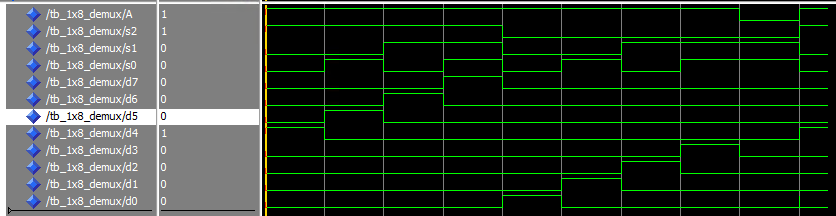
\includegraphics[width=\textwidth]{./diagrams/1x8_demux_simulation.png}
\end{figure}

\begin{figure}[h]
\caption{1x8 de-multiplexer from structural modeling wave graph}
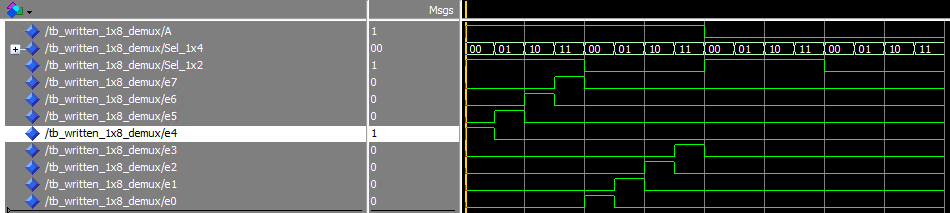
\includegraphics[width=\textwidth]{./diagrams/written_1x8_demux_simulation.png}
\end{figure}

\begin{table}[h]
    \begin{tabular}{|c|c|c||c|c|c|c|c|c|c|c|}
        \hline
        \multicolumn{3}{|c||}{Inputs} & \multicolumn{8}{c|}{Outputs} \\
        \hline
        \( s_2 \) & \( s_1 \) & \( s_0 \) & \( i_7 \) & \( i_6 \) & \( i_5 \) & \( i_4 \) & \( i_3 \) & \( i_2 \) & \( i_1 \) & \( i_0 \) \\
        \hline
        0 & 0 & 0 & A & 0 & 0 & 0 & 0 & 0 & 0 & 0 \\
        \hline
        0 & 0 & 1 & 0 & A & 0 & 0 & 0 & 0 & 0 & 0 \\
        \hline
        0 & 1 & 0  & 0 & 0 & A & 0 & 0 & 0 & 0 & 0 \\
        \hline
        0 & 1 & 1  & 0 & 0 & 0 & A & 0 & 0 & 0 & 0 \\
        \hline
        1 & 0 & 0  & 0 & 0 & 0 & 0 & A & 0 & 0 & 0 \\
        \hline
        1 & 0 & 1  & 0 & 0 & 0 & 0 & 0 & A & 0 & 0 \\
        \hline
        1 & 1 & 0  & 0 & 0 & 0 & 0 & 0 & 0 & A & 0 \\
        \hline
        1 & 1 & 1  & 0 & 0 & 0 & 0 & 0 & 0 & 0 & A \\
        \hline
    \end{tabular}
    \caption{Truth table for 1x8 demux using 1x2 and 1x4 demux}
\end{table}

The Truth table when compared against the wave simulation graphs is identical in the appropriate outputs such as when taking the 3-bit binary string (100) in either of the simulations the output would be $i_4$ and that is because the simulation as well as the VHDL code version followed the logic derived from the boolen equation and by extension the truth table from which the equation was derived. The difference between the code generated by the circuit diagram and the code I wrote were drastically different and I feel as though--with bias of course--that my code was much more concise on how the 1x2 and 1x4 demuxes played a role in building the 1x8 demux meanwhile the generated VHDL was more spaghetti like with its many "SYNTHESIZED WIRE" calls. It was apparent that the code generated needed a clear visual of what was going on or it would take quite some time to understand the logic from just the code.

\clearpage
%-------------------- 3x8 decoder begin --------------------
\section{Exercise C: 3-to-8 Decoder}
\subsection{Objective}
The purpose of this exercise was to create a 3x8 decoder circuit from its respective combinational logic, deepening our knowledge of the way in which circuits could be derived from their respective boolean equation, and by extension their truth table. Inclusively, the exercise seeks to further enhance our understanding of writing VHDL codea long with designing circuits and test benches.

\subsection{Functionality and Specifications}

\begin{figure}[h]
    \begin{multline}
        \\y_0 = i_2'i_1'i_0' \\
        y_1 = i_2'i_1'i_0 \\
        y_2 = i_2'i_1i_0' \\
        y_3 = i_2'i_1i_0 \\
        y_4 = i_2i_1'i_0' \\
        y_5 = i_2i_1'i_0 \\
        y_6 = i_2i_1i_0' \\
        y_7 = i_2i_1i_0 \\
    \end{multline}
    \caption{3x8 decoder boolean eq.}
\end{figure}

\noindent The boolean equation and by extension the truth table both show the behavior of the decoder. Whenever a 3-bit input is inputted which consists of $i_2$, $i_1$, and $i_0$ the output would be that number represented in 8 bits (1 byte). Hence if the incoming encoded input was 000 the encoder would return 00000001 with $y_7$ being the MSB. 

\begin{figure}[h]
\caption{3x8 decoder}
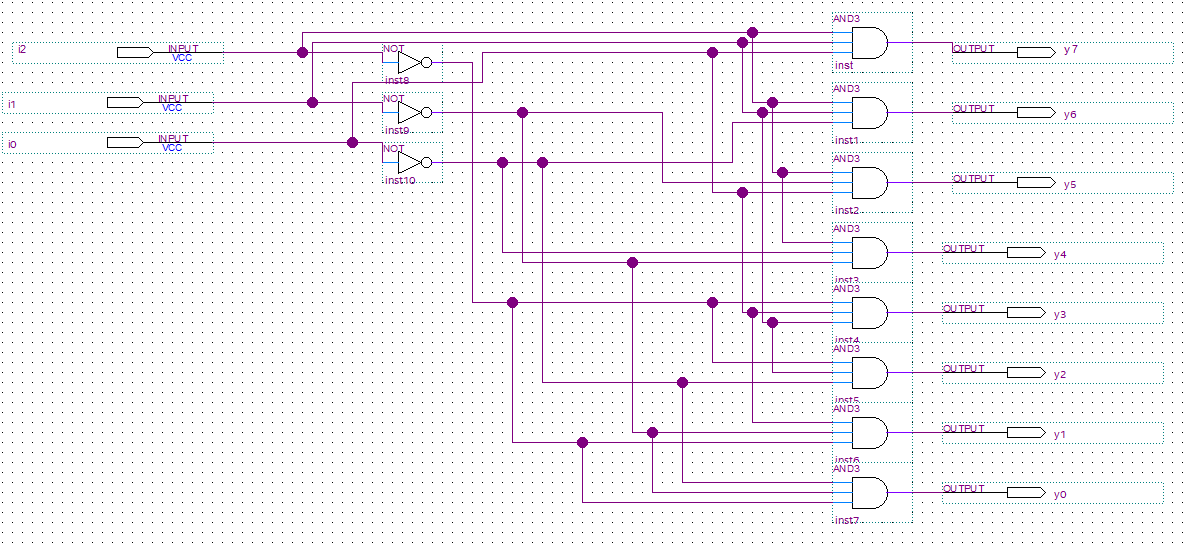
\includegraphics[width=\textwidth]{./diagrams/3x8_decoder.png}
\end{figure}
\subsubsection{VHDL Code generated from the design file}
\begin{minted}[linenos]{vhdl}
    LIBRARY ieee;
    USE ieee.std_logic_1164.all; 
    
    LIBRARY work;
    
    ENTITY lab_assign_1 IS 
    	PORT
    	(
    		i2 :  IN  STD_LOGIC;
    		i1 :  IN  STD_LOGIC;
    		i0 :  IN  STD_LOGIC;
    		y7 :  OUT  STD_LOGIC;
    		y6 :  OUT  STD_LOGIC;
    		y5 :  OUT  STD_LOGIC;
    		y4 :  OUT  STD_LOGIC;
    		y3 :  OUT  STD_LOGIC;
    		y2 :  OUT  STD_LOGIC;
    		y1 :  OUT  STD_LOGIC;
    		y0 :  OUT  STD_LOGIC
    	);
    END lab_assign_1;
    
    ARCHITECTURE bdf_type OF lab_assign_1 IS 
    
    SIGNAL	SYNTHESIZED_WIRE_12 :  STD_LOGIC;
    SIGNAL	SYNTHESIZED_WIRE_13 :  STD_LOGIC;
    SIGNAL	SYNTHESIZED_WIRE_14 :  STD_LOGIC;
    
    
    BEGIN 
    
    y7 <= i2 AND i1 AND i0;    
    y6 <= i2 AND i1 AND SYNTHESIZED_WIRE_12;

    SYNTHESIZED_WIRE_12 <= NOT(i0);
    y5 <= i2 AND SYNTHESIZED_WIRE_13 AND i0;
    y4 <= i2 AND SYNTHESIZED_WIRE_12 AND SYNTHESIZED_WIRE_13;
    y3 <= SYNTHESIZED_WIRE_14 AND i0 AND i1;
    y2 <= SYNTHESIZED_WIRE_14 AND i1 AND SYNTHESIZED_WIRE_12;
    y1 <= i0 AND SYNTHESIZED_WIRE_13 AND SYNTHESIZED_WIRE_14;
    y0 <= SYNTHESIZED_WIRE_12 AND SYNTHESIZED_WIRE_13 AND SYNTHESIZED_WIRE_14;
    
    SYNTHESIZED_WIRE_14 <= NOT(i2);
    SYNTHESIZED_WIRE_13 <= NOT(i1);
    END bdf_type;

\end{minted}

\subsubsection{VHDL Code generated from the design file}
\begin{minted}[linenos]{vhdl}
    library IEEE;
    use IEEE.STD_LOGIC_1164.ALL;
    
    entity written_3x8_decoder is
        Port ( A : in  STD_LOGIC_VECTOR(2 downto 0);
               Y : out  STD_LOGIC_VECTOR(7 downto 0));
    end written_3x8_decoder;
    
    architecture Behavioral of written_3x8_decoder is
    begin
        process(A)
        begin
            case A is
                when "000" => Y <= "00000001";
                when "001" => Y <= "00000010";
                when "010" => Y <= "00000100";
                when "011" => Y <= "00001000";
                when "100" => Y <= "00010000";
                when "101" => Y <= "00100000";
                when "110" => Y <= "01000000";
                when "111" => Y <= "10000000";
                when others => Y <= "00000000"; 
            end case;
        end process;
    end Behavioral;
\end{minted}


\subsubsection{VHDL code for Test bench}
\begin{minted}[linenos]{vhdl}
    library IEEE;
    use IEEE.STD_LOGIC_1164.ALL;
    use IEEE.STD_LOGIC_TEXTIO.ALL;
    use std.textio.all;
    
    entity tb_3x8_decoder is
    end tb_3x8_decoder;
    
    architecture test of tb_3x8_decoder is
        signal i2 :  STD_LOGIC;
        signal i1 :  STD_LOGIC;
        signal i0 :  STD_LOGIC;
        signal y7 :  STD_LOGIC;
        signal y6 :  STD_LOGIC;
        signal y5 :  STD_LOGIC;
        signal y4 :  STD_LOGIC;
        signal y3 :  STD_LOGIC;
        signal y2 :  STD_LOGIC;
        signal y1 :  STD_LOGIC;
        signal y0 :  STD_LOGIC;
    
        component lab_assign_1
    	Port
    	(
    		i2 :  IN  STD_LOGIC;
    		i1 :  IN  STD_LOGIC;
    		i0 :  IN  STD_LOGIC;
    		y7 :  OUT  STD_LOGIC;
    		y6 :  OUT  STD_LOGIC;
    		y5 :  OUT  STD_LOGIC;
    		y4 :  OUT  STD_LOGIC;
    		y3 :  OUT  STD_LOGIC;
    		y2 :  OUT  STD_LOGIC;
    		y1 :  OUT  STD_LOGIC;
    		y0 :  OUT  STD_LOGIC
    	);
        end component;
    
    begin
        uut: lab_assign_1 port map(i2, i1, i0, y7, y6, y5, y4, y3, y2, y1,y0);
        PROCESS
        BEGIN
            i2 <= '0';
            i1 <= '0';
            i0 <= '0';
            WAIT for 10 ns;
            i0 <= '1';
            WAIT for 10 ns;
            i1 <= '1';
            i0 <= '0';
            WAIT for 10 ns;
            i0 <= '1';
            WAIT for 10 ns;
            i2 <= '1';
            i1 <= '0';
            i0 <= '0';
            WAIT for 10 ns;
            i0 <= '1';
            WAIT for 10 ns;
            i1 <= '1';
            i0 <= '0';
            WAIT for 10 ns;
            i0 <= '1';
            WAIT for 10 ns;
        END PROCESS;
    
    end test;
\end{minted}

\subsubsection{written VHDL code Test bench}
\begin{minted}[linenos]{vhdl}
    library IEEE;
    use IEEE.STD_LOGIC_1164.ALL;
    
    entity tb_written_3x8_decoder is
    end tb_written_3x8_decoder;
    
    architecture test of tb_written_3x8_decoder is
        component written_3x8_decoder
            Port ( A : in  STD_LOGIC_VECTOR(2 downto 0);
                   Y : out  STD_LOGIC_VECTOR(7 downto 0));
        end component;
    
        signal A : STD_LOGIC_VECTOR(2 downto 0);
        signal Y : STD_LOGIC_VECTOR(7 downto 0);
    
    begin
    
        UUT: written_3x8_decoder port map (
            A,
            Y
        );
    
        process
        begin
            A <= "000"; 
            wait for 10 ns;
            
            A <= "001";
            wait for 10 ns;
            
            A <= "010"; 
            wait for 10 ns;
            
            A <= "011"; 
            wait for 10 ns;
            
            A <= "100"; 
            wait for 10 ns;
            
            A <= "101"; 
            wait for 10 ns;
            
            A <= "110"; 
            wait for 10 ns;
       
            A <= "111"; 
            wait for 10 ns;
            
            wait;
        end process;
    end test;

\end{minted}

\subsection{Simulation}
\begin{figure}[h]
\caption{3x8 decoder wave simulation}
\centering
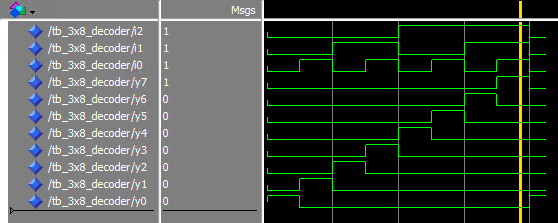
\includegraphics[width=\textwidth]{./diagrams/3x8_simulation.png}
\end{figure}

\subsection{Simulation}
\begin{figure}[h]
\caption{written 3x8 decoder wave simulation}
\centering
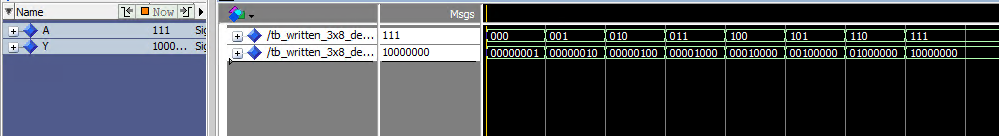
\includegraphics[width=\textwidth]{./diagrams/written_3x8_decoder_simulation.png}
\end{figure}

\begin{table}[h]
    \begin{tabular}{|c|c|c||c|c|c|c|c|c|c|c|}
        \hline
        \multicolumn{3}{|c||}{Inputs} & \multicolumn{8}{c|}{Outputs} \\
        \hline
        \( i_2 \) & \( i_1 \) & \( i_0 \) & \( y_7 \) & \( y_6 \) & \( y_5 \) & \( y_4 \) & \( y_3 \) & \( y_2 \) & \( y_1 \) & \( y_0 \) \\
        \hline
        0 & 0 & 0 & 1 & 0 & 0 & 0 & 0 & 0 & 0 & 0 \\
        \hline
        0 & 0 & 1 & 0 & 1 & 0 & 0 & 0 & 0 & 0 & 0 \\
        \hline
        0 & 1 & 0  & 0 & 0 & 1 & 0 & 0 & 0 & 0 & 0 \\
        \hline
        0 & 1 & 1  & 0 & 0 & 0 & 1 & 0 & 0 & 0 & 0 \\
        \hline
        1 & 0 & 0  & 0 & 0 & 0 & 0 & 1 & 0 & 0 & 0 \\
        \hline
        1 & 0 & 1  & 0 & 0 & 0 & 0 & 0 & 1 & 0 & 0 \\
        \hline
        1 & 1 & 0  & 0 & 0 & 0 & 0 & 0 & 0 & 1 & 0 \\
        \hline
        1 & 1 & 1  & 0 & 0 & 0 & 0 & 0 & 0 & 0 & 1 \\
        \hline
    \end{tabular}
    \caption{Truth table for 3x8 decoder}
\end{table}

\noindent Similar to the 1x8 demux the truth table and the wave graph simulation essentially mirror each other. When taking a closer look the plot we see there is almost a staircase that forms as the time elapses and the inputs change, when they are starting from input 000, we see that the graph peaks at $y_0$ similar to the binary string that is generated when this encoded input is passed into the circuit. 

%-------------------- 3x8 decoder END --------------------
\clearpage
%-------------------- 8x3 p-encoder begin --------------------
\section{Exercise D: 8-to-3 Priority Encoder}
\subsection{Objective}
The purpose of this exercise was to create a 8x3 priority encoder circuit from its respective combinational logic. Now having compiled and generated the relevant VHDL for the circuit one was able to simulate the circuit in action. Thus resulting in a better understanding of designing a 8x3 priority encoder circuit from its respective combinational equation, and testing that created circuit.

\subsection{Functionality and Specifications}

\begin{figure}[h]
\caption{8x3 priority encoder}
\centering
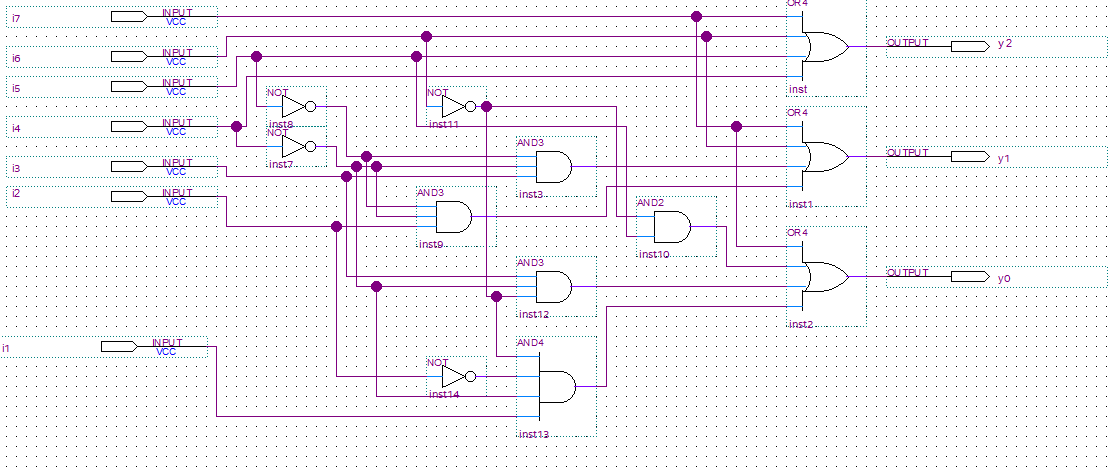
\includegraphics[width=\textwidth]{./diagrams/8x3_penc_design.png}
\end{figure}

\begin{figure}[h]
    \begin{multline}
        \\y_2 = i_4+i_5+i_6+i_7 \\
        y_1 = (i_3+i_2)i_4'i_5'+i_6+i_7 \\
        y_0 = i_7+i_5i_6'+i_3i_4'i_6'+i_1i_2'i_4'i_6' \\
    \end{multline}
    \caption{8x3 priority encoder boolean eq.}
\end{figure}

\noindent Here in the case of our priority encoder we see that for the 8 bits that are inputted the input with the highest priority we will be output hence the nomenclature of priority encoding. This is also reflected in the boolean equation that was derived from its corresponding truth table. Taking as an example output $y_2$ that only is dependent on whether $i_4$, $i_5$, $i_6$, or $i_7$ it is observed in the truth table that the only times $y_2$ is 1 is whenever these 4 inputs have priority which makes sense since they are the 4 highest priorities and $y_2$ is the MSB.



{VHDL code generated from design file}
\begin{minted}[linenos]{vhdl}
    LIBRARY ieee;
    USE ieee.std_logic_1164.all; 
    
    LIBRARY work;
    
    ENTITY \8x3_p_enc\ IS 
    	PORT
    	(
    		i2 :  IN  STD_LOGIC;
    		i1 :  IN  STD_LOGIC;
    		i3 :  IN  STD_LOGIC;
    		i4 :  IN  STD_LOGIC;
    		i5 :  IN  STD_LOGIC;
    		i6 :  IN  STD_LOGIC;
    		i7 :  IN  STD_LOGIC;
    		y2 :  OUT  STD_LOGIC;
    		y1 :  OUT  STD_LOGIC;
    		y0 :  OUT  STD_LOGIC
    	);
    END \8x3_p_enc\;
    
    ARCHITECTURE bdf_type OF \8x3_p_enc\ IS 
    
    SIGNAL	SYNTHESIZED_WIRE_0 :  STD_LOGIC;
    SIGNAL	SYNTHESIZED_WIRE_1 :  STD_LOGIC;
    SIGNAL	SYNTHESIZED_WIRE_15 :  STD_LOGIC;
    SIGNAL	SYNTHESIZED_WIRE_16 :  STD_LOGIC;
    SIGNAL	SYNTHESIZED_WIRE_6 :  STD_LOGIC;
    SIGNAL	SYNTHESIZED_WIRE_8 :  STD_LOGIC;
    SIGNAL	SYNTHESIZED_WIRE_9 :  STD_LOGIC;
    SIGNAL	SYNTHESIZED_WIRE_10 :  STD_LOGIC;
    SIGNAL	SYNTHESIZED_WIRE_17 :  STD_LOGIC;
    
    
    BEGIN 
    
    
    
    y2 <= i7 OR i5 OR i4 OR i6;
    
    
    y1 <= i7 OR SYNTHESIZED_WIRE_0 OR SYNTHESIZED_WIRE_1 OR i6;
    
    
    SYNTHESIZED_WIRE_10 <= SYNTHESIZED_WIRE_15 AND i5;
    
    
    SYNTHESIZED_WIRE_15 <= NOT(i6);
    
    
    
    SYNTHESIZED_WIRE_8 <= i3 AND SYNTHESIZED_WIRE_16 AND SYNTHESIZED_WIRE_15;
    
    
    SYNTHESIZED_WIRE_9 <= SYNTHESIZED_WIRE_15 AND SYNTHESIZED_WIRE_6 AND SYNTHESIZED_WIRE_16 AND i1;
    
    
    SYNTHESIZED_WIRE_6 <= NOT(i2);
    
    
    
    y0 <= i7 OR SYNTHESIZED_WIRE_8 OR SYNTHESIZED_WIRE_9 OR SYNTHESIZED_WIRE_10;
    
    
    SYNTHESIZED_WIRE_0 <= SYNTHESIZED_WIRE_17 AND SYNTHESIZED_WIRE_16 AND i3;
    
    
    SYNTHESIZED_WIRE_16 <= NOT(i4);
    
    
    
    SYNTHESIZED_WIRE_17 <= NOT(i5);
    
    
    
    SYNTHESIZED_WIRE_1 <= SYNTHESIZED_WIRE_17 AND SYNTHESIZED_WIRE_16 AND i2;
    
    
    END bdf_type;

\end{minted}

\subsubsection{written VHDL code}
\begin{minted}[linenos]{vhdl}
    library IEEE;
    use IEEE.STD_LOGIC_1164.ALL;
    
    entity written_8x3_penc is
        Port ( I : in  STD_LOGIC_VECTOR(7 downto 0);  --
               Y : out  STD_LOGIC_VECTOR(2 downto 0); 
               V : out STD_LOGIC                     
             );
    end written_8x3_penc;
    
    architecture Behavioral of written_8x3_penc is
    begin
        process(I)
        begin
            V <= '0';
            Y <= "000";
           
            case I is
                when "10000000" => Y <= "111"; V <= '1';
                when "01000000" => Y <= "110"; V <= '1';
                when "00100000" => Y <= "101"; V <= '1';
                when "00010000" => Y <= "100"; V <= '1';
                when "00001000" => Y <= "011"; V <= '1';
                when "00000100" => Y <= "010"; V <= '1';
                when "00000010" => Y <= "001"; V <= '1';
                when "00000001" => Y <= "000"; V <= '1';
                when others => V <= '0'; -- no valid input passed!!!
            end case;
        end process;
    end Behavioral;
\end{minted}


\subsubsection{VHDL code for Test bench}
\begin{minted}[linenos]{vhdl}
    library IEEE;
    use IEEE.STD_LOGIC_1164.ALL;
    use IEEE.STD_LOGIC_TEXTIO.ALL;
    use std.textio.all;
    
    entity tb_8x3_p_encoder is
    end tb_8x3_p_encoder;
    
    architecture test of tb_8x3_p_encoder is
        signal i1 : STD_LOGIC;
        signal i2 : STD_LOGIC;
        signal i3 : STD_LOGIC;
        signal i4 : STD_LOGIC;
        signal i5 : STD_LOGIC;
        signal i6 : STD_LOGIC;
        signal i7 : STD_LOGIC;
        signal y2 : STD_LOGIC;
        signal y1 : STD_LOGIC;
        signal y0 : STD_LOGIC;
    
        component \8x3_p_enc\
            Port ( i1 : in STD_LOGIC;
                   i2 : in STD_LOGIC;
                   i3 : in STD_LOGIC;
                   i4 : in STD_LOGIC;
                   i5 : in STD_LOGIC;
                   i6 : in STD_LOGIC;
                   i7 : in STD_LOGIC;
                   y2 : out STD_LOGIC;
                   y1 : out STD_LOGIC;
    	       y0 : out STD_LOGIC);
        end component;
    
    begin
        uut: \8x3_p_enc\ port map(i1, i2, i3, i4, i5, i6, i7, y2, y1, y0);
        PROCESS
        BEGIN
    	-- No inputs active
            i1 <= '0';
            i2 <= '0';
            i3 <= '0';
            i4 <= '0';
            i5 <= '0';
            i6 <= '0';
            i7 <= '0';
            WAIT for 20 ns;
            -- i1 active
            i1 <= '1';
            i2 <= '0';
            i3 <= '0';
            i4 <= '0';
            i5 <= '0';
            i6 <= '0';
            i7 <= '0';
            WAIT for 20 ns;
            -- i2 active
            i1 <= '0';
            i2 <= '1';
            i3 <= '0';
            i4 <= '0';
            i5 <= '0';
            i6 <= '0';
            i7 <= '0';
            WAIT for 20 ns;
            -- i3 active
            i1 <= '0';
            i2 <= '0';
            i3 <= '1';
            i4 <= '0';
            i5 <= '0';
            i6 <= '0';
            i7 <= '0';
            WAIT for 20 ns;
            -- i4 active
            i1 <= '0';
            i2 <= '0';
            i3 <= '0';
            i4 <= '1';
            i5 <= '0';
            i6 <= '0';
            i7 <= '0';
            WAIT for 20 ns;
            -- i5 active
            i1 <= '0';
            i2 <= '0';
            i3 <= '0';
            i4 <= '0';
            i5 <= '1';
            i6 <= '0';
            i7 <= '0';
            WAIT for 20 ns;
            -- i6 active
            i1 <= '0';
            i2 <= '0';
            i3 <= '0';
            i4 <= '0';
            i5 <= '0';
            i6 <= '1';
            i7 <= '0';
            WAIT for 20 ns;
            -- i7 active
            i1 <= '0';
            i2 <= '0';
            i3 <= '0';
            i4 <= '0';
            i5 <= '0';
            i6 <= '0';
            i7 <= '1';
            WAIT for 20 ns;
            -- multiple active, output should be: (Highest priority, i7)
            i1 <= '0';
            i2 <= '0';
            i3 <= '1';
            i4 <= '0';
            i5 <= '1';
            i6 <= '0';
            i7 <= '1';
            WAIT for 20 ns;
            -- multiple active, output should be: (Highest priority, i6)
            i1 <= '1';
            i2 <= '1';
            i3 <= '1';
            i4 <= '1';
            i5 <= '0';
            i6 <= '1';
            i7 <= '0';
            WAIT for 20 ns;
            -- multiple active, output should be: (Highest priority, i5)
            i1 <= '1';
            i2 <= '1';
            i3 <= '1';
            i4 <= '1';
            i5 <= '1';
            i6 <= '0';
            i7 <= '0';
            WAIT for 20 ns;
            -- multiple active, output should be: (Highest priority, i4)
            i1 <= '1';
            i2 <= '1';
            i3 <= '1';
            i4 <= '1';
            i5 <= '0';
            i6 <= '0';
            i7 <= '0';
            WAIT for 20 ns;
            -- multiple active, output should be: (Highest priority, i3)
            i1 <= '1';
            i2 <= '1';
            i3 <= '1';
            i4 <= '0';
            i5 <= '0';
            i6 <= '0';
            i7 <= '0';
            WAIT for 20 ns;
            -- multiple active, output should be: (Highest priority, i2)
            i1 <= '1';
            i2 <= '1';
            i3 <= '0';
            i4 <= '0';
            i5 <= '0';
            i6 <= '0';
            i7 <= '0';
            WAIT for 20 ns;
    
        END PROCESS;
    
    end test;

\end{minted}

\subsubsection{written VHDL code Test bench}
\begin{minted}{vhdl}
    library IEEE;
    use IEEE.STD_LOGIC_1164.ALL;
    
    entity tb_written_8x3_penc is
    end tb_written_8x3_penc;
    
    architecture test of tb_written_8x3_penc is
        component written_8x3_penc
            Port ( I : in  STD_LOGIC_VECTOR(7 downto 0);
                   Y : out  STD_LOGIC_VECTOR(2 downto 0);
                   V : out STD_LOGIC );
        end component;
    
        signal I : STD_LOGIC_VECTOR(7 downto 0);
        signal Y : STD_LOGIC_VECTOR(2 downto 0);
        signal V : STD_LOGIC;
    
    begin
        UUT: written_8x3_penc port map (
            I,
            Y,
            V
        );
    
        process
        begin
            I <= "10000000"; wait for 10 ns;
            I <= "01000000"; wait for 10 ns;
            I <= "00100000"; wait for 10 ns;
            I <= "00010000"; wait for 10 ns;
            I <= "00001000"; wait for 10 ns;
            I <= "00000100"; wait for 10 ns;
            I <= "00000010"; wait for 10 ns;
            I <= "00000001"; wait for 10 ns;
            I <= "00000000"; wait for 10 ns;
            wait;
        end process;
    end test;

\end{minted}


\subsection{Simulation}
\begin{figure}[h]
\caption{8x3 priority encoder wave graph}
\centering
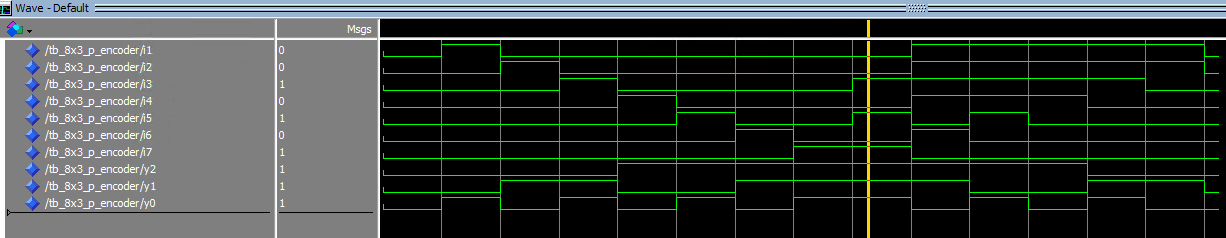
\includegraphics[width=\textwidth]{./diagrams/8x3_p_enc_simulation.png}
\end{figure}

\begin{figure}[h]
\caption{written 8x3 priority encoder wave graph}
\centering
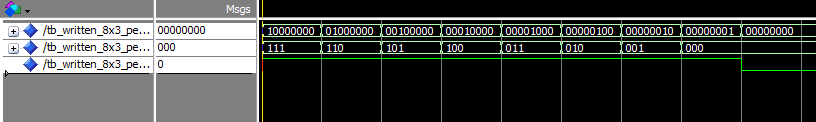
\includegraphics[width=\textwidth]{./diagrams/written_8x3_penc.png}
\end{figure}

\begin{table}[h]
    \begin{tabular}{|c|c|c|c|c|c|c|c||c|c|c|}
        \hline
        \multicolumn{8}{|c}{Inputs} & \multicolumn{3}{c|}{Outputs} \\
        \hline
        \( i_7 \) & \( i_6 \) & \( i_5 \) & \( i_4 \) & \( i_3 \) & \( i_2 \) & \( i_1 \) & \( i_0 \) & \( y_2 \) & \( y_1 \) & \( y_0 \) \\
        \hline
        0 & 0 & 0 & 0 & 0 & 0 & 0 & 0 & X & X & X \\
        \hline
        0 & 0 & 0 & 0 & 0 & 0 & 0 & 1 & 0 & 0 & 0 \\
        \hline
        0 & 0 & 0 & 0 & 0 & 0 & 1 & X & 0 & 0 & 1 \\
        \hline
        0 & 0 & 0 & 0 & 0 & 1 & X & X & 0 & 1 & 0 \\
        \hline
        0 & 0 & 0 & 0 & 1 & X & X & X & 0 & 1 & 1 \\
        \hline
        0 & 0 & 0 & 1 & X & X & X & X & 1 & 0 & 0 \\
        \hline
        0 & 0 & 1 & X & X & X & X & X & 1 & 0 & 1 \\
        \hline
        0 & 1 & X & X & X & X & X & X & 1 & 1 & 0 \\
        \hline
        1 & X & X & X & X & X & X & X & 1 & 1 & 1 \\
        \hline
    \end{tabular}
    \caption{Truth table for 3x8 decoder}
\end{table}

\noindent As represented by the wave simulation graph it is apparent that the truth table also reflects its contents as shown in cases with $i_1$,..$i_7$ where we have the don't cares which could be any bit and still not change the output. The reason, why in the truth table we also have don't cares on the side of outputs--and more specifically when we have the case of the 00000000 binary string be input is that in this case there is essentially no priority given and so none can be selected. Hence why our simulation begins at 000000000 and there are no rises in the graph but when we introduce the binary string 0000001X we finally get an output of 001 which is seen in the bottom portion of the graph correctly reflecting what is in the truth table.


%-------------------- 8x3 p-encoder END --------------------
\clearpage
%-------------------- SR latch & Flip flop begin --------------------
\section{Exercise E: Set-Reset Flip-Flop \& D Flip-Flop (Positive Edge Trigger)}
\subsection{Objective}

\subsection{Simulation}
%-------------------- SR latch & Flip flop END --------------------

\section{Conclusions}

\end{document}